\documentclass[11pt,a4paper]{article}
\usepackage[hyperref]{style/emnlp-ijcnlp-2019}
\usepackage{times}
\usepackage{latexsym}
\usepackage{url}
\usepackage{graphicx,subfigure}
\usepackage{bm,bbm}
\usepackage{amsmath}
\usepackage{enumitem}
\usepackage{multirow}

\usepackage{xspace}
\usepackage{CJKutf8}
\usepackage{xpinyin}
\usepackage{footnote}
\usepackage{threeparttable}

\aclfinalcopy % Uncomment this line for the final submission

%\setlength\titlebox{5cm}
% You can expand the titlebox if you need extra space
% to show all the authors. Please do not make the titlebox
% smaller than 5cm (the original size); we will check this
% in the camera-ready version and ask you to change it back.

\setlength{\tabcolsep}{2pt}
\makesavenoteenv{table}

\newcommand{\ch}[1]{\begin{CJK*}{UTF8}{gbsn}#1\end{CJK*}}

\newcommand{\explain}[2]{\underbrace{#2}_{\mbox{\footnotesize{#1}}}}

\newcommand{\abr}[1]{\textsc{#1}}

% Use these comment definitions to see paper without comments
\newcommand{\jbgcomment}[1]{}
\newcommand{\wycomment}[1]{}
\newcommand{\psrcomment}[1]{}
\newcommand{\psrnewcomment}[1]{}
\newcommand{\ignore}[1]{}

% Use these comment definitions to keep comments visible
%\newcommand{\jbgcomment}[1]{ \textcolor{blue}{[JBG: {\bf #1}]} }
%\newcommand{\wycomment}[1]{ \textcolor{red}{[WY: {\bf #1}]} }
%\newcommand{\psrcomment}[1]{ \textcolor{green}{[PSR: {\bf #1}]} }
%\newcommand{\psrnewcomment}[1]{ \textcolor{olive}{[PSR: {\bf #1}]} }

% Math
\newcommand{\prob}[2]{\Pr \left( #1 \,|\, #2 \right)}
\newcommand{\ind}[1]{\mathbbm{1} \left( #1 \right)}
\newcommand{\rhost}{$\bm{\rho_{S \rightarrow T}}$\xspace}
\newcommand{\rhots}{$\bm{\rho_{T \rightarrow S}}$\xspace}

% Names
\newcommand{\lda}{\textsc{lda}\xspace}
\newcommand{\mtm}{\textsc{mtm}\xspace}
\newcommand{\mtms}{\textsc{mtm}s\xspace}
\newcommand{\ptlda}{pt\textsc{lda}\xspace}

\newcommand{\paco}{\textsc{paco}\xspace}
\newcommand{\inco}{\textsc{inco}\xspace}
\newcommand{\en}{\textsc{en}\xspace}
\newcommand{\zh}{\textsc{zh}\xspace}
\newcommand{\si}{\textsc{si}\xspace}
\newcommand{\tr}{\textsc{tr}\xspace}

\newcommand{\us}{\textsc{us}\xspace}

\newcommand{\lbfgs}{\textsc{l-bfgs}\xspace}
\newcommand{\pmi}{\textsc{pmi}\xspace}
\newcommand{\tfidf}{\textsc{tf-idf}\xspace}
\newcommand{\mtanchor}{MTAnchor\xspace}
\newcommand{\mcta}{\textsc{mcta}\xspace}
\newcommand{\cca}{\textsc{cca}\xspace}

\newcommand{\intra}{\textsc{in}\xspace}
\newcommand{\cross}{\textsc{cr}\xspace}
\newcommand{\toplink}{\textsc{top}\xspace}

% Table commands
\newcommand{\tabincell}[2]{\begin{tabular}{@{}#1@{}}#2\end{tabular}}

%\newcommand\BibTeX{B{\sc ib}\TeX}

% Note: The PDFLaTeX-compiled document contains unembedded fonts due to the two Visio-generated PDF figures contain unembedded fonts.
% The error message is "Your PDF document contains some fonts that are not embedded. This is not allowed as per the submission guidelines".
% The way to resolve this is to run the following commands in the figures directory:
%    pdftops mtm.pdf
%    ps2pdf14 -dPDFSETTINGS=/prepress mtm.ps mtm2.pdf
%    pdftops topic_link_vertical.pdf
%    ps2pdf14 -dPDFSETTINGS=/prepress topic_link_vertical.ps topic_link_vertical2.pdf

\title{A Multilingual Topic Model for\\ Learning Weighted Topic Links Across Corpora with Low Comparability}

\author{Weiwei Yang\thanks{\hspace{0.2cm}Now at Facebook}\\
  Computer Science \\
  \\
  University of Maryland \\
  {\tt wwyang@cs.umd.edu} \And
  Jordan Boyd-Graber\thanks{\hspace{0.2cm}Now at Google Research Z\"urich} \\
  Computer Science, iSchool, \\
  Language Science, \abr{umiacs} \\
  University of Maryland \\
   {\tt jbg@umiacs.umd.edu}
  \And
  Philip Resnik \\
  Linguistics and \abr{umiacs} \\
  \\
  University of Maryland \\
  {\tt resnik@umd.edu} \\}

\date{}

\begin{document}

\maketitle

\begin{abstract}
  Multilingual topic models (\mtms) learn topics on documents in
  multiple languages.
  Past models align topics across languages by implicitly assuming the
  documents in different languages are highly comparable, often a false
  assumption.
  We introduce a new model that does not rely on this assumption,
  particularly useful in important low-resource language scenarios.
  Our \mtm learns weighted topic links and connects cross-lingual
  topics only when the dominant words defining them are similar,
  outperforming \lda and previous \mtms in classification tasks using
  documents' topic posteriors as features.
  It also learns coherent topics on documents with low
  comparability.

\jbgcomment{Coming back to Philip's earlier points, if we wanted to
  change title to remove ``incomparable'', now we're able to. \wycomment{Done.}}

\end{abstract}


\section{Introduction}
\label{sec:intro}

Topic models explain document collections at a high
level~\cite{boyd-graber-2017-topic-model-book}.
%
Multilingual topic models (\mtms) uncover latent topics \emph{across}
languages and reveal
%The latent topics---represented as distributions over
%words---summarize documents and help analysts discover trends~\cite{lau-2012-tm-trend}, analyze
%emotions~\cite{bao-2009-tm-emotions}, or recommend content~\cite{marlin-2003-tm-cf}.\jbgcomment{Add some monolingual
%  citations here, perhaps changing the applications.}\wycomment{Done.}
%In contrast to monolingual topic models, \mtms reveal
commonalities and differences across languages
and cultures~\cite{ni-2009-mtm-wiki,shi-2016-mtm-common,gutierrez-2016-mtm-diff}.
Existing models extend latent Dirichlet
allocation~\cite[\lda]{blei-2003-lda} and learn \emph{aligned} topics
across languages~\cite{mimno-2009-plda}.

Prior models work well because they implicitly assume---even if not part of the
model---parallel or highly comparable data with well-aligned topics.
%
However, this
assumption does not always comport with reality.
%
Even documents from the same place and time
can discuss very different things across languages: in multicultural
London, Hindi tweets focus on a Bollywood actor's
\abr{bbc} appearance, French blogs fret
about Brexit, and English articles focus on Tottenham's lineup.
%
Generally, corpora have a range of ``nonparallelness''~\citep{fung-2000-bilingual-stat}.
%
In less comparable settings,
% Even in a ``comparable'' setting,
%consideration of multiple languages brings to the forefront the fact that,
while some topics are shared, languages' emphasis may diverge
and some topics may lack analogs.

% Unfortunately, it is not always the case that the cross-lingual
% documents are highly comparable or parallel. Even on the same topic,
% the documents in different languages may talk about different
% aspects. For instance, in the news articles about
% \underline{Earthquake}, we find that the English articles talk about
% the worldwide earthquakes, while the Chinese articles focus on the
% earthquake happened in Sichuan Province in 2008. Such difference in
% topics and topic aspects can fail a \mtm which aligns all topics,
% because they do not let people know which topics are shared across
% languages and which are unique in a language.


\begin{figure}[t]
  \centering
  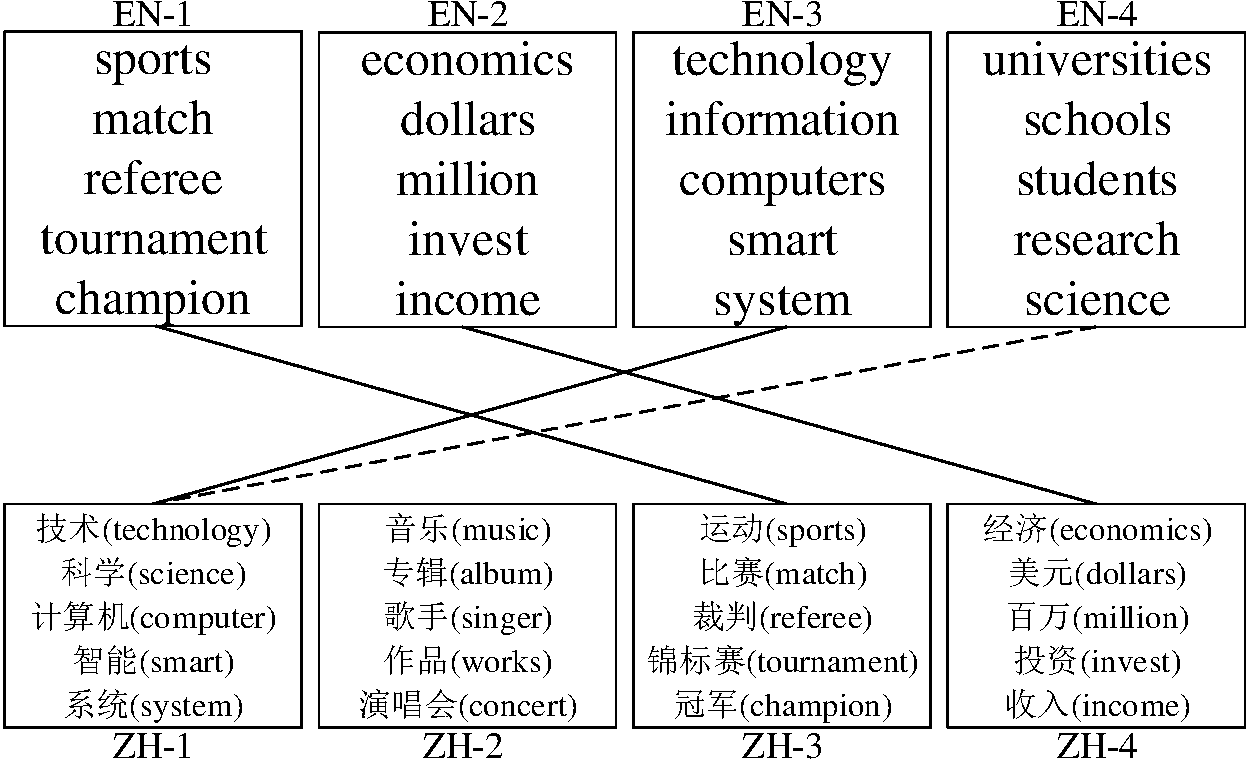
\includegraphics[width=.96\linewidth]{2019_emnlp_mtm/figures/topic_link_vertical2.pdf}
  \caption{\ignore{Our \mtm learns weighted topic links: }Topic pairs
    with many word translation pairs have high link weights, e.g.,
    (\en-1, \zh-3) and (\en-2, \zh-4); topic pairs with partial
    overlap receive lower weights, e.g., (\en-4, \zh-1); a topic is
    unlinked if there is no corresponding topic in the other language
    (\zh-2).\jbgcomment{We're not using the full width of the figure, and the Hanzi are very skinny; try to use the width to at least get a topic label in for the Chinese topics.  Otherwise it's not very useful to someone who doesn't speak Chinese\wycomment{Done.}}
  }\label{fig:topic_link_example}
\end{figure}


We therefore introduce a new multilingual topic model that assumes
each language has its own topic sets and jointly learns all topics,
but does not force one-to-one alignment across languages.
%
Instead, our \mtm learns \emph{weighted} topic links across languages
and only assigns a high link weight to a topic pair whose top words
have many direct translation pairs
(Figure~\ref{fig:topic_link_example}).
%, so they are weakly linked, while \zh-1 is strongly linked with \en-4.
Moreover, it allows unlinked topics if there is no matching topic in
the other language. This makes the model robust for (more common)
less-comparable data with topic misalignment.
%
Joint inference also allows insights from
high-resource languages to uncover low-resource language patterns. It is particularly useful
in scenarios that involve modeling topics on low-resource languages in humanitarian assistance, peacekeeping,
and/or infectious disease response, while limiting the additional cost to other steps that will also need to be taken,
such as finding or creating a word translation dictionary.

\psrnewcomment{Reference to humanitarian assistance felt out of
  place. \jbgcomment{Would be good to add back in now that we have
    more space, connect better to LORELEI.} \wycomment{Done.}}

% We describe our \mtm in the bilingual case which has a language~$S$ with $K_S$ topics and another language~$T$ with $K_T$ topics, and it is fairly easy to generalize it to multilingual. The \mtm has two matrices~\rhots and~\rhost that store topic link weight matrices and convert the topics from language~$T$ to~$S$ and~$S$ to~$T$ respectively. For a translation pair, its two words have the same sense, so the topics in which the two words are assigned high probability mass are likely to be corresponding topics of each other in the two languages. Therefore, the values of~$\bm{\rho}$'s are learned through converting the words' topic distributions in one language into the topic space of the other language using~$\bm{\rho}$'s and making them as close as possible to their translation words' topic distributions in the other language (see Section~\ref{sec:model}). In this process, the shared topic pairs across languages will get higher weights, while a unique topic in a language will have a high-entropy weight distribution over the topics in the other language.

We validate the \mtm in two classification tasks using
inferred topic posteriors as features.
%
Our \mtm has higher F1 than other models in both intra- and
cross-lingual evaluations, while discovering coherent topics and
meaningful topic links.


%\section{Posterior Regularizers to Inject Knowledge}
\label{sec:post_reg}

Improving topic models often requires modeling additional information:
word correlations~\cite{boyd-graber-2007-tm-wsd}, document
labels~\cite{mcauliffe-2008-slda}, or document
links~\cite{chang-2010-rtm}.
%
Likewise, linking multilingual topics requires an infusion of
knowledge, either in the form of word translations~\cite{Hu-2014-ptlda}, paired documents~\cite{mimno-2009-plda},
or embeddings~\cite{das-2015-glda,ammar-2016-uw-embed}.
\wycomment{It looks like no work is done on linking multilingual topics using word embeddings. Shall we cite multilingual word embedding and monolingual Gaussian LDA? 
\jbgcomment{For camera ready, better to add citations wherever relevant}}
However, increasing the complexity of the model often comes at a cost:
inference becomes more complicated.  Posterior regularization becomes
an effective middle ground.  It's relatively flexible but able to model many
forms of metadata.

\newcite{yang-2015-knowledge} specifically apply posterior
regularization to Gibbs sampling~\cite{heinrich-09} for
vanilla topic models that sample only token topic
assignments~$\bm{z}$.
For each prior knowledge source~$m$ in the knowledge set~$M$, they
create a potential function $f_m (\bm{z}, \bm{w}, \bm{d})$ of topic assignments~$\bm{z}$,
words~$\bm{w}$, and/or documents~$\bm{d}$.
Higher $f_m (\bm{z}, \bm{w}, \bm{d})$ indicates better consistency
with~$m$ at the current state.  The posterior regularizer is
\begin{equation}\label{equ:post_reg}
\Psi \left( \bm{z}, \bm{w}, M \right) = \prod_{m \in M} \exp \left( f_m (\bm{z}, \bm{w}, \bm{d}) \right),
\end{equation}
which they include in the collapsed Gibbs sampling equation
as:\par\nobreak
\begin{align}
\Pr ( &z_{d,n}=k \,|\, \bm{z_{-d,n}}, w_{d,n}=v, \bm{w_{-d,n}} ) \notag\\
\propto & \explain{\textsc{lda} Sampling}{ \left( N_{d,k}^{-d,n}+\alpha \right) \frac{N_{k,v}^{-d,n}+\beta}{N_{k,\cdot}^{-d,n}+V\beta}} \notag\\
& \explain{Posterior Regularizer}{\Psi \left( z_{d,n}=k, \bm{z_{-d,n}}, \bm{w}, M \right)}, \label{equ:gibbs_post_reg}
\end{align}
where $N_{d,k}$ is the number of tokens in document~$d$ assigned to
topic~$k$; $N_{k,v}$ is the number of times that word~$v$ is assigned
to topic~$k$; and $\cdot$ denotes marginal counts; $^{-d,n}$ means
that the count excludes the token~\cite{heinrich-09,resnik-2010-gibbs}.\jbgcomment{Now that we have more time, ease into Gibbs sampling a little bit more.  Give intuition about what sampling step does, how the additional term changes things with an example (beyond just saying ``consistent with''.}

In this formulation, the potential functions shape Gibbs sampling
inference: topic assignments are more likely when they are consistent
with the prior knowledge included in the potential functions.
This brings significant flexibility in the expression of the potential
function $f_m (\bm{z}, \bm{w}, \bm{d})$.
The expression is not restricted to probabilistic distributions,
exponential family, or conjugacy.  \jbgcomment{``conjugacy'' isn't specific enough.  Need to say ``conjugate priors''}
It can be expressed flexibly using the combinations of \emph{any} of
the values from topic assignments, words, and/or documents. 
\jbgcomment{This is a little too much; you could make the computation
  too expensive to be done tractibly.  Would be good to reign this in
  a little bit.}
Moreover, changing the expressions of potential functions does not
change the main structure of the topic model or require full
re-derivation of the Gibbs sampling equation, which allows more
flexible experimentation.

For our \mtm, we encode the topic link weights and the translation
pairs' topic distributions into the posterior regularizer. Thus we can
convey prior knowledge across languages and improve the topic models
for the two languages.


\section{Multilingual Topic Model for Connecting Cross-Lingual Topics}
%\section{Model}
\label{sec:model}


%\begin{figure}[t!]
%  \centering
%  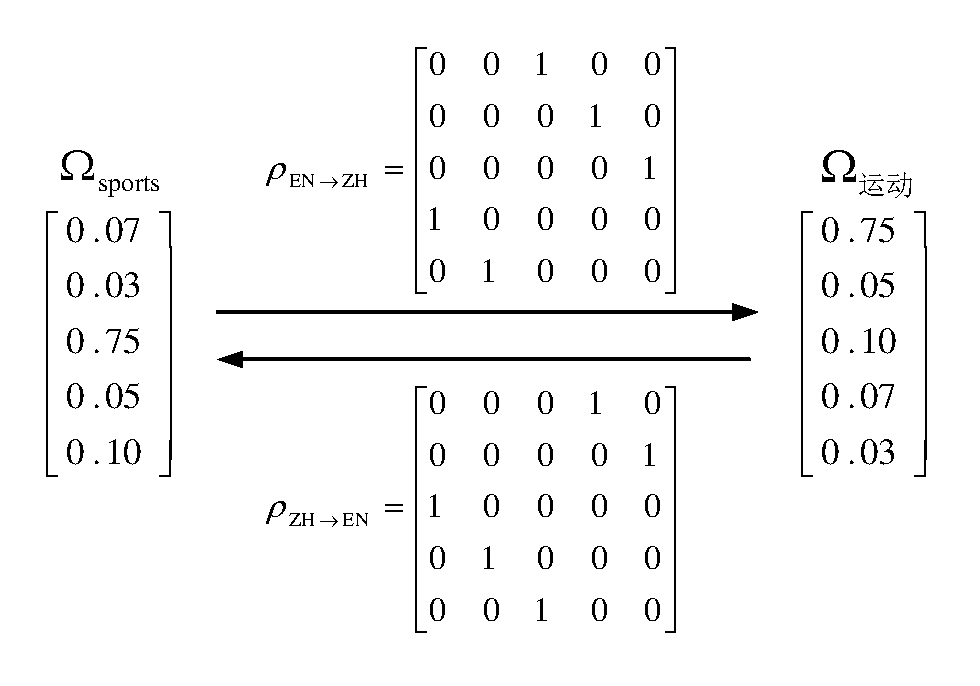
\includegraphics[width=.935\linewidth]{2019_emnlp_mtm/figures/rho.pdf}
%  \caption{Our model uses topic link weight matrices~$\bm{\rho}$'s to
%    transform topics from one language to another.  Unlike other
%    models, it allows a topic to linked to another topic or multiple topics.}
%
%  \label{fig:rho}
%\end{figure}

\newcite{yang-2015-knowledge} present a flexible framework for adding
regularization to topic models.  We extend this model to the
multilingual setting by adding a potential function that links topics
across languages.  For simplicity of exposition, we focus on the
bilingual case with languages~$S$ and~$T$.


\jbgcomment{I think this contrast could be a little clearer.  All of the models there are monolingual, etc.  It's not just that there are two matrices\dots \wycomment{Is it better now?}}

Unlike~\newcite{yang-2015-knowledge} that encode monolingual information only, our potential function encodes multilingual knowledge parameterized
by two matrices,~\rhost and~\rhots, that transform topics between the two languages.
Cells' values are between 0 and 1 and a cell $\rho_{S \rightarrow T, k_T, k_S}$ close to one is a strong connection of topics~$k_T$ and~$k_S$ in language~$T$ and~$S$.  \jbgcomment{``while transforming'' is vague; make clearer. \wycomment{Looks like it is clearer if not mentioning transformation.}}
Transformations~$\bm{\rho}$ are learned from translation pairs' topic
distributions.

These topic distributions come from the assignments of Gibbs
sampling~\cite{griffiths-2004-lda-gibbs}.
%
Fortunately adding the potential function is equivalent to adding an
additional term to Gibbs sampling for topic
models~\cite{yang-2015-knowledge}.
%
During sampling, each token is assigned
to a topic, so we can compute a \emph{post
  hoc} word distribution over topics. The probability of a topic~$k$ given a word~$w$ is $\prob{k}{w} \equiv \Omega_{w,k}
\equiv N_{k,w} / N_w$, where~$N_{k,w}$ is the number of times that
word~$w$ is assigned to topic~$k$ and~$N_w$ is~$w$'s term frequency.

\jbgcomment{Expand this out a little bit; explicitly say that this is
  the probability of topic given a word. \wycomment{Done.}}

To find good topic links~\rhost, we use a dictionary.
%
For instance, given the translation pair of ``sports'' and ``\ch{运动}
(\pinyin{yun4} \pinyin{dong4})'', they should have similar topic distributions, so we want $\bm{\rho_{\text{\en}
    \rightarrow \text{\zh}}} \bm{\Omega_{\text{sports}}}$ to be
close to $\bm{\Omega_{\text{\ch{运动}}}}$ and vice versa. \jbgcomment{Make this clearer: these words should have similar topics.\wycomment{Done.}}
%
Moreover, the transformations should be symmetric:  $\bm{\rho_{S
    \rightarrow T}} \bm{\Omega_{w_S}}$ close to~$\bm{\Omega_{w_T}}$,
and vice versa. \jbgcomment{Explaing what ``consistent'' means with words: one transform should be the inverse of the other.\wycomment{Maybe ``symmetric'' is a better word here?}}
We encode this cross-lingual
knowledge of topic transformations into the potential function~$\Psi$ which measures the difference of translation pairs' topic distributions after transformation\ignore{as the reciprocal product
of all translation pairs' topic distribution distances after
transformation by~$\bm{\rho}$}:  \jbgcomment{Explain with words what this equation is trying to do; don't just say ``close to''.\wycomment{Done.}}
\begin{equation}
\small
\left( \prod_{c=1}^{C} \left\lVert \bm{\Omega_{S,c}} - \bm{\rho_{T \rightarrow S}} \bm{\Omega_{T,c}} \right\rVert_{2}^{\eta_c} \left\lVert \bm{\rho_{S \rightarrow T}} \bm{\Omega_{S,c}} - \bm{\Omega_{T,c}} \right\rVert_{2}^{\eta_c} \right)^{-1}, \label{equ:psi}
\end{equation}
where~$\eta_c$ is the statistical importance of the~$c$-th translation pair to the corpus \jbgcomment{``importance'' is vague, rename or be more specific. \wycomment{Elaborated a little bit. Is it better?}}
(Figure~\ref{fig:mtm_model}, full
details in the Supplement).
\begin{figure}[t]
  \centering
  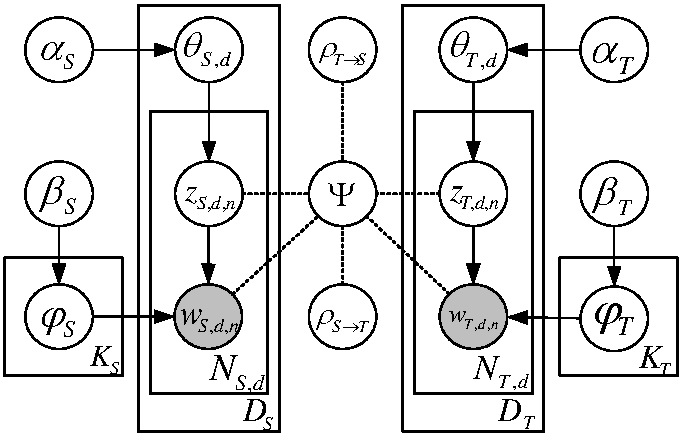
\includegraphics[width=\linewidth]{2019_emnlp_mtm/figures/mtm2.pdf}
  \caption{The graphical model of our multilingual topic model. The
    topic links~$\bm{\rho}$, as instantiated by the function $\Psi$,
    encourage topics to encourage word translations to have
    consistent topics.}
\label{fig:mtm_model}
\end{figure}

\ignore{
:\par\nobreak
\begin{small}
\begin{enumerate}[leftmargin=*,noitemsep]
  \item For each topic $k \in \{ 1, \ldots, K_T \}$ in language~$T$
  \begin{enumerate}
    \item Draw word distribution $\bm{\phi_{T,k}} \sim \text{Dir} (\beta_T)$.
  \end{enumerate}
  \item For each document $d \in \{ 1, \ldots, D_T \}$ in language~$T$
  \begin{enumerate}
    \item Draw topic distribution $\bm{\theta_{T, d}} \sim \text{Dir} (\alpha_T)$.
    \item For each token $t_{T,d,n}$ in document~$d$
    \begin{enumerate}
      \item Draw a topic $z_{T,d,n} \sim \text{Mult} (\bm{\theta_{T,d}})$.
      \item Draw a word $w_{T,d,n} \sim \text{Mult} (\bm{\phi_{T,z_{T,d,n}}})$.
    \end{enumerate}
  \end{enumerate}
  \item For each topic $k \in \{ 1, \ldots, K_S \}$ in language~$S$
  \begin{enumerate}
    \item Draw word distribution $\bm{\phi_{S,k}} \sim \text{Dir} (\beta_S)$.
  \end{enumerate}
  \item For each document $d \in \{ 1, \ldots, D_S \}$ in language~$S$
  \begin{enumerate}
    \item Draw topic distribution $\bm{\theta_{S,d}} \sim \text{Dir} (\alpha_S)$.
    \item For each token $t_{S,d,n}$ in document $d$
    \begin{enumerate}
      \item Draw a topic $z_{S,d,n} \sim \text{Mult} (\bm{\theta_{S,d}})$.
      \item Draw a word $w_{S,d,n} \sim \text{Mult} (\bm{\phi_{S,z_{S,d,n}}})$.
    \end{enumerate}
  \end{enumerate}
  \item Draw the posterior regularizer~$\Psi$ with Equation~\ref{equ:psi}.
\end{enumerate}
\end{small}
}

\jbgcomment{Make it clearer that the models there don't have additional parameters, but we do (and say what those parameters are).\wycomment{Done.}}
While~\newcite{yang-2015-knowledge} provide a blueprint for Gibbs
sampling with potential functions without additional parameters,
our model has additional parameters of~\rhost and~\rhots so we need to optimize them.
Thus, we use stochastic
\textsc{em}~\cite{celeux-1985-sem}. The E-step updates tokens'
topic assignments using Gibbs sampling, while holding the parameters of the
topic link weight matrices~$\bm{\rho}$ fixed.
%\footnote{The equations in E-step and the optimization
%  for~\rhots in M-step are available in Supplement.}
The M-step optimizes~$\bm{\rho}$ while holding the topic
assignments fixed. We\jbgcomment{I would instead say that you optimize in log space\wycomment{Done.}}
optimize~$\Psi$ in log space using the objective
function~$J(\bm{\rho_{S \rightarrow T}})$ as
\begin{equation}\label{equ:rho_obj}
\small
\sum_{c=1}^{C} \eta_c \log \left\lVert \bm{\Omega_{T,c}} - \bm{\rho_{S \rightarrow T, i_T}} \bm{\Omega_{S,c}} \right\rVert_{2},
\end{equation}
which is minimized by using \lbfgs~\cite{liu-1989-lbfgs}, with the
partial derivatives with respect to~$\rho_{S \rightarrow T, k_T, k_S}$
\begin{equation}\label{equ:rho_grad}
\small
- \sum_{c=1}^{C} \frac {\eta_c \Omega_{S,c,k_S} \left( \Omega_{T,c,k_T} - \bm{\rho_{S \rightarrow T, k_T}} \bm{\Omega_{S,c}} \right)} {\left\lVert \bm{\Omega_{T,c}} - \bm{\rho_{S \rightarrow T, i_T}} \bm{\Omega_{S,c}} \right\rVert_{2}^2}.
\end{equation}


\section{Experiments}
\label{sec:exp}

We evaluate our model extrinsically on classification tasks,
followed by intrinsic topic coherence.

\subsection{Classification with Topic Posteriors}
\label{subsec:exp_class}

%\begin{table}[t]
%  \centering
%  \small
%  \begin{threeparttable}
%  \begin{tabular}{lrrrr}
%    Method & \en-\intra & \si/\zh-\intra & \en-\cross & \si/\zh-\cross \\ \hline \hline
%    \multicolumn{5}{c}{Disaster Response} \\ \hline
%    \mcta\tnote{\dag} & 12.99 & 26.53 & 4.08 & 15.58 \\
%    \mtanchor\tnote{\dag} & 20.78 & 32.65 & 24.49 & 24.68 \\
%    \lda & 27.78 & 24.01 & 22.86 & 21.05 \\
%    \ptlda & 12.77 & 18.18 & 16.01 & 15.09 \\ \hline
%    \mtm & \textbf{42.86} & 23.08 & 22.22 & 26.67 \\
%    \mtm + \toplink & \textbf{42.86} & 23.08 & \textbf{35.29} & \textbf{33.33} \\
%    \mtm + \tfidf & 26.67 & \textbf{38.10} & 14.46 & 15.09 \\
%    \mtm + \tfidf + \toplink & 26.67 & \textbf{38.10} & 14.46 & 11.43 \\ \hline \hline
%    \multicolumn{5}{c}{Wikipedia} \\ \hline
%    \mcta\tnote{\dag} & 51.56 & 33.35 & 23.24 & 39.79 \\
%    \mtanchor\tnote{\dag} & 80.71 & 75.33 & 57.62 & 54.54 \\
%    \lda & 92.08 & 83.37 & 16.52 & 10.46 \\
%    \ptlda & 91.58 & 83.33 & 2.85 & 21.02 \\ \hline
%    \mtm & 92.98 & \textbf{86.48} & 74.69 & 64.48 \\
%    \mtm + \toplink & 92.98 & \textbf{86.48} & \textbf{78.13} & \textbf{83.08} \\
%    \mtm + \tfidf & \textbf{94.07} & 85.59 & 57.27 & 55.06 \\
%    \mtm + \tfidf + \toplink & \textbf{94.07} & 85.59 & 63.20 & 59.64 \\ \hline \hline
%  \end{tabular}
%  \caption{Our \mtm outperforms all the baselines in intra- and cross-lingual evaluations in F1 scores.}\label{tab:class}
%  \begin{tablenotes}
%    \item[\dag] Reported by~\newcite{yuan-2018-mtanchor}.  \jbgcomment{Would be good to have error bars on these if possible (can we also try a bar chart?)}
%  \end{tablenotes}
%  \end{threeparttable}
%\end{table}

\begin{figure}[t]
  \centering
  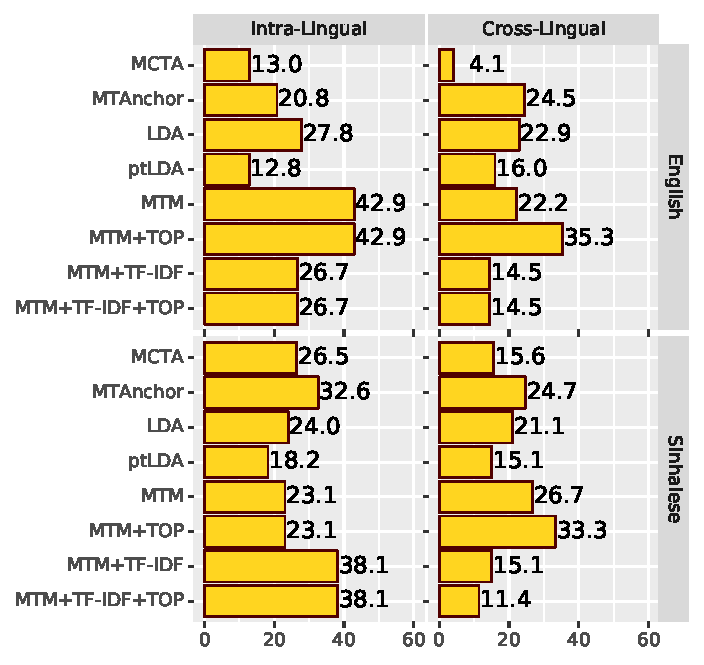
\includegraphics[width=\linewidth]{2019_emnlp_mtm/auto_fig/lorelei.pdf}
  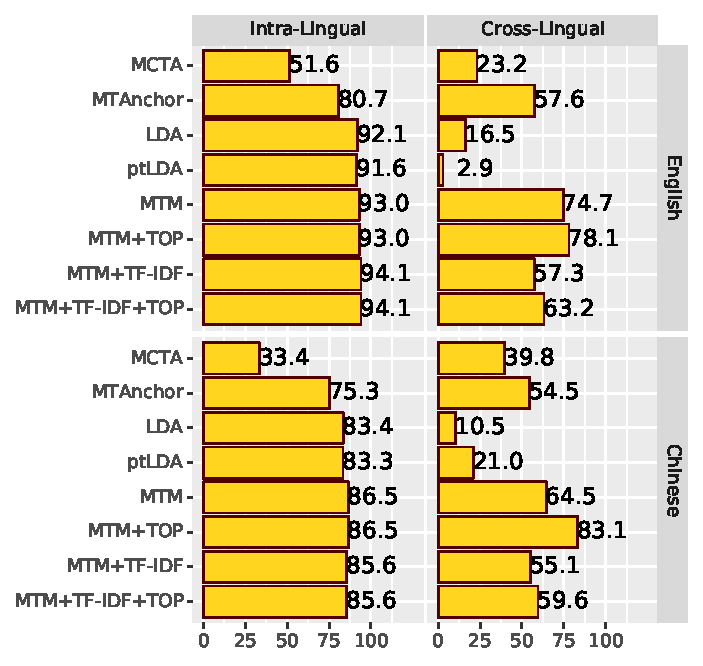
\includegraphics[width=\linewidth]{2019_emnlp_mtm/auto_fig/wiki.pdf}
  \caption{The F1 scores on disaster response (upper) and Wikipedia (lower) datasets. Our \mtm outperforms all the baselines in intra- and cross-lingual evaluations.\wycomment{It's hard to obtain the error bars. The datasets are just split into a training set and a test set, not cross-validation.}}\label{fig:f1}
\end{figure}

\jbgcomment{It seems that we never explicitly define the features.
  Did that get deleted?  Let's make sure that's explained at least at
  a high level here. \wycomment{We just never explicitly define them. I added it in the second paragraph.}}

We use two datasets for classification: Wikipedia documents in English (\en)
 and Chinese (\zh)~\cite{yuan-2018-mtanchor} and an
English-Sinhalese (\si) disaster response
dataset~\cite{strassel-2016-lorelei}.\footnote{More dataset details in
  the Supplement.}
%
Each dataset provides labeled documents and a
dictionary. \newcite{yuan-2018-mtanchor} extract the \en-\zh
dictionary from \textsc{mdbg}, while~\newcite{strassel-2016-lorelei}
construct the \en-\si dictionary from online resources and manual
annotation.\footnote{\textsc{mdbg}:
  \url{https://www.mdbg.net/chinese/dictionary?page=cc-cedict}}
%
Each Wikipedia document is labeled with one of the topics of
\emph{film}, \emph{music}, \emph{animals}, \emph{politics},
\emph{religion}, and \emph{food}. A portion of the disaster response
documents are labeled with one of eight types of needed rescue
resources: \emph{evacuation}, \emph{food supply},
\emph{search/rescue}, \emph{utilities}, \emph{infrastructure},
\emph{medical assistance}, \emph{shelter}, and \emph{water supply}.

We follow~\newcite{yuan-2018-mtanchor} for preprocessing (such as lemmatization for English and segmentation for Chinese) and use a linear \textsc{svm}
for classification.
%
For the Wikipedia dataset, we
report micro-F1 scores on a six-way classification.
 For the disaster response dataset, our goal is binary classification of
the need for \emph{evacuation} versus other assistance.
The classification uses features of topic posteriors: $\prob{k}{d} \equiv N_{d,k} / N_{d}$ which is the proportion of the tokens assigned to topic~$k$ in document~$d$.

The baselines include polylingual tree
\lda~\cite[\ptlda]{Hu-2014-ptlda} which encodes the dictionary as a
tree prior~\cite{andrzejewski-2009-dir-forest}, Multilingual Topic
Anchoring~\cite[\mtanchor]{yuan-2018-mtanchor}, and Multilingual
Cultural-common Topic Analysis~\cite[\mcta]{shi-2016-mtm-common}. We
also include \lda, which runs monolingually in each language. We use
20 topics and set hyper-parameters $\alpha=0.1$ and $\beta=0.01$
(if applicable).

Our evaluations are both intra- and cross-lingual. The intra-lingual
evaluation trains and tests classifiers on the same
language, while the cross-lingual evaluation trains
classifiers on one language and tests on another. In cross-lingual
evaluations, \mtanchor, \mcta, and \ptlda align topic spaces, so topic
posterior transformation is not necessary. \lda cannot transform topic
spaces, so we do not apply any transformation. For our \mtm, we
explore two transformation methods with~$\bm{\rho}$. The first
multiplies~$\bm{\rho}$ with a language's document topic distributions,
i.e.,
$\bm{\rho_{\text{\zh}\rightarrow \text{\en}}}
\bm{\theta_{\text{\zh}}}$ and vice versa. The second (\toplink),
transfers each document topic's probability mass to the topic in the
other language with the highest link weight.\footnote{An example of \toplink is available in the Supplement.}

Our \mtm has higher F1 both intra- and cross-lingually
(Figure~\ref{fig:f1}).\ignore{\footnote{\mtanchor and \mcta results
    are reported by~\newcite{yuan-2018-mtanchor}.}} \tfidf weighting
on translation pairs sometimes improves the intra-lingual F1,
although it hurts the cross-lingual F1. Connecting the top
linked topics (\toplink) is better than directly using the topic link
weight matrices. This indicates that~$\bm{\rho}$'s values have
some noise.

\jbgcomment{There should be a clearer transition here that says that
  the topics are aligned across languages; let's see if they make
  sense.\wycomment{Done.}}

\subsection{Looking at Learned Topics}
\label{subsec:exp_example}

\psrnewcomment{I've updated the subsection heading to make it clearer that this is example/analysis, not evaluation}

%\begin{table*}[t!]
%  \centering
%  \small
%  \begin{tabular}{lll}
%    Model & Language & Words \\ \hline \hline
%    \multirow{3}{*}{\mcta} & \zh & \multirow{3}{*}{
%        \begin{tabular}{lllllll}
%            \ch{主演} & \ch{改编} & \ch{本} & \ch{小说} & \ch{拍摄} & \ch{角色} & \ch{战士} \\
%            starring & adapt & this & novel & shoot & role & fighter \\
%            dog & san & movie & mexican & figher & novel & california
%        \end{tabular}} \\
%     & \zh-\tr & \\ \cline{2-3}
%     & \en & \\ \hline
%    \multirow{3}{*}{\mtanchor} & \zh & \multirow{3}{*}{
%        \begin{tabular}{lllllll}
%            \ch{主演} & \ch{改编} & \ch{饰演} & \ch{本片} & \ch{演员} & \ch{编剧} & \ch{讲述} \\
%            starring & adapt & act & this movie & actor & playwright & narrate \\
%            kong & hong & movie & official & martial & box & reception
%        \end{tabular}} \\
%     & \zh-\tr & \\ \cline{2-3}
%     & \en & \\ \hline
%    \multirow{3}{*}{\lda} & \zh & \multirow{3}{*}{
%        \begin{tabular}{lllllll}
%            \ch{电影} & \ch{部} & \ch{美国} & \ch{上映} & \ch{英语} & \ch{剧情} & \ch{片} \\
%            movie & movie quantifier & USA & release & English & plot & movie \\
%            film & star & direct & release & action & plot & character
%        \end{tabular}} \\
%     & \zh-\tr & \\ \cline{2-3}
%     & \en & \\ \hline
%    \multirow{3}{*}{\ptlda} & \zh & \multirow{3}{*}{
%        \begin{tabular}{lllllll}
%            \ch{电影} & \ch{胶片} & \ch{星} & \ch{动作} & \ch{释放} & \ch{影片} & \ch{剧情} \\
%            movie & film & star & action & release & movie & plot \\
%            film & star & direct & action & release & plot & write
%        \end{tabular}} \\
%     & \zh-\tr & \\ \cline{2-3}
%     & \en & \\ \hline
%    \multirow{5}{*}{\mtm} & \zh & \multirow{5}{*}{
%        \begin{tabular}{lllllll}
%            \ch{电影} & \ch{部} & \ch{上映} & \ch{动画} & \ch{故事} & \ch{作品} & \ch{英语} \\
%            movie & movie quantifier & release & animation & story & works & English \\
%            film & direct & star & release & action & plot & production \\
%            kill & find & death & attack & escape & return & back \\
%            shrine & japanese & temple & japan & shinto & kami & god
%        \end{tabular}} \\
%     & \zh-\tr & \\ \cline{2-3}
%     & \en-1 (0.20) & \\
%     & \en-2 (0.12) & \\
%     & \en-3 (0.11) & \\ \hline
%    \multirow{5}{*}{\tabincell{l}{\mtm +\\ \tfidf}} & \zh & \multirow{5}{*}{
%        \begin{tabular}{lllllll}
%            \ch{电影} & \ch{部} & \ch{上映} & \ch{美国} & \ch{英语} & \ch{导演} & \ch{片} \\
%            movie & movie quantifier & release & USA & English & director & movie \\
%            film & direct & star & action & release & plot & movie \\
%            film & kill & find & escape & attack & return & back \\
%            character & series & star & game & trek & create & episode
%        \end{tabular}} \\
%     & \zh-\tr & \\ \cline{2-3}
%     & \en-1 (0.32) & \\
%     & \en-2 (0.24) & \\
%     & \en-3 (0.09) & \\ \hline
%  \end{tabular}
%  \caption{The topics of \underline{Movies} given by models. \zh-\tr indicates the English translations of the Chinese words. For the Chinese topics given by our \mtm, the top three English topics and their link weights are also given.}\label{tab:example}
%\end{table*}

\begin{table}[t!]
  \centering
  \small
  \begin{tabular}{ll}
    Lang. & Words \\ \hline \hline
    \multicolumn{2}{c}{\mcta} \\ \hline
    \multirow{2}{*}{\zh} & \ch{主演} (starring), \ch{改编} (adapt), \ch{本} (this), \\
     & \ch{小说} (novel), \ch{拍摄} (shoot), \ch{角色} (role) \\
    \en & dog, san, movie, mexican, fighter, novel \\ \hline \hline
    \multicolumn{2}{c}{\mtanchor} \\ \hline
    \multirow{2}{*}{\zh} & \ch{主演} (starring), \ch{改编} (adapt), \ch{饰演} (act), \\
     & \ch{本片} (the movie), \ch{演员} (actor), \ch{编剧} (playwright) \\
    \en & kong, hong, movie, official, martial, box \\ \hline \hline
    \multicolumn{2}{c}{\lda} \\ \hline
    \multirow{2}{*}{\zh} & \ch{电影} (movie), \ch{部} ([Q] movie),\footnote{In Tables~\ref{tab:example} and~\ref{tab:topic_links}, ``[Q]'' denotes the Chinese word is a counter for the following English word.} \ch{美国} (USA), \\
     & \ch{上映} (release), \ch{英语} (English), \ch{剧情} (plot) \\
    \en & film, star, direct, release, action, plot \\ \hline \hline
    \multicolumn{2}{c}{\ptlda} \\ \hline
    \multirow{2}{*}{\zh} & \ch{电影} (movie), \ch{胶片} (film), \ch{星} (star), \\
     & \ch{动作} (action), \ch{释放} (release), \ch{影片} (movie) \\
    \en & film, star, direct, action, release, plot \\ \hline \hline
    \multicolumn{2}{c}{\mtm} \\ \hline
    \multirow{2}{*}{\zh} & \ch{电影} (movie), \ch{部} ([Q] movie), \ch{上映} (release),  \\
     & \ch{动画} (animation), \ch{故事} (story), \ch{作品} (works),  \\
    \en (.20) & film, direct, star, release, action, plot \\
    \en (.12) & kill, find, death, attack, escape, return \\
    \en (.11) & shrine, japanese, temple, japan, shinto, kami \\ \hline \hline
    \multicolumn{2}{c}{\mtm + \tfidf} \\ \hline
    \multirow{2}{*}{\zh} & \ch{电影} (movie), \ch{部} ([Q] movie), \ch{上映} (release),  \\
     & \ch{美国} (USA), \ch{英语} (English), \ch{导演} (director) \\
    \en (.32) & film, direct, star, action, release, plot \\
    \en (.24) & film, kill, find, escape, attack, return \\
    \en (.09) & character, series, star, game, trek, create \\ \hline \hline
  \end{tabular}
  \caption{The \underline{Movies} topics given by models. For the Chinese (\zh) topics given by \mtm, the top three English (\en) topics and their link weights are also given.\wycomment{I cut the number of top words from 7 to 6 to save space as the last word does not affect the evaluation much.}}\label{tab:example}
\end{table}

Past \mtms align topics across languages but our \mtm does not, so we compare the topics across models to see how they differ.
We look at the \underline{Movies} topics from the Wikipedia dataset (Table~\ref{tab:example}). For the Chinese \mtm topics, we show the three English topics with the highest link weights.

The topics are about \underline{Movies}, but the \mcta and \mtanchor
topics do not rank ``movie'' or ``\ch{电影} (\pinyin{dian4}
\pinyin{ying3})'' at the top.
%
The \ptlda topics, although aligned
well, incorrectly align\jbgcomment{``problems'' is vague, be specific\wycomment{Done.}} some Chinese words. ``\ch{胶片}
(\pinyin{jiao1} \pinyin{pian4})'' means ``\emph{photographic}
film'',\ignore{instead of ``movie''} while ``\ch{释放}
(\pinyin{shi4} \pinyin{fang4})'' means \emph{release} as in ``let something go'', not movie distribution.
%
\ptlda links words based on translations without looking at the
context, which causes problems with multiple-sense words.
%
The \lda and \mtm topics are generally coherent.

\psrnewcomment{I am shifting the emphasis in this paragraph to be more
  about the topics, since the topic \emph{links} are the focus of the
  next subsection.}

The \mtm's unique joint modeling of weighted topic links also recovers
additional topical structure: after linking respective \en-\zh
\underline{Movies} topics,\jbgcomment{It's unclear what ``we
  find'' means here; let's tighten up wording\wycomment{Done.}} the next linked topics are
\underline{Action Movies} (``kill'', ``death'', ``attack'', and
``escape'').
%
Further, the models capture a degree of connection between
\underline{Movies} and \underline{Computer Games} (\mtm + \tfidf) and
\underline{Japanese Animations} (\mtm).
%
\psrnewcomment{Is ``unique joint modeling'' accurate? I'm trying to
  focus here on the jointness of the model producing the topics rather
  than the links, which are in the next subsection. Also, I'm kind of
  on the fence on saying anything about the 3rd-ranked links. We're
  trying to put a positive spin on it, but I could also see these
  being interpreted as stretching it a little to far or just
  incorrect. Either way, we're kind of begging the question of how far
  down the link-weights list you set your cutoff of what's relevant or
  not. One could possibly hedge this by adding the word ``arguably'',
  to say ``Further the models arguably capture a degree of...'' so at
  least it's clear we know we're stretching it a little
  bit. \wycomment{I think the phrasing and to focus on the joint
    modeling are good. I added more info to address its uniqueness.}}


\subsection{Looking at Learned Topic Links}
\label{subsec:exp_topic_link}

\psrnewcomment{I've updated the subsection heading to make it clearer that this is example/analysis, not evaluation}

%\begin{table*}[t!]
%  \centering
%  \small
%  \begin{tabular}{lrl}
%    Language & Weight & Words \\ \hline \hline
%    \zh-0 & -- & \multirow{4}{*}{
%        \begin{tabular}{lllllll}
%            \ch{学名} & \ch{它们} & \ch{呈} & \ch{白色} & \ch{长} & \ch{黑色} & \ch{厘米} \\
%            scientific name & they & show & white & long & black & centimeter \\
%            specie & bird & eagle & genus & white & owl & black\\
%            breed & chicken & white & goose & bird & black & list
%        \end{tabular}} \\
%    \zh-0-\tr & -- &  \\
%    \en-12 & 0.57 &  \\
%    \en-19 & 0.13 &  \\ \hline
%    \zh-14 & -- & \multirow{4}{*}{
%        \begin{tabular}{lllllll}
%            \ch{主义} & \ch{组织} & \ch{美国} & \ch{革命} & \ch{运动} & \ch{政府} & \ch{人民} \\
%            -ism & organization & USA & evolution & campaign & government & people \\
%            sex & law & act & sexual & marriage & court & legal \\
%            traffic & victim & government & trafficking & child & force & country
%        \end{tabular}} \\
%    \zh-14-\tr & -- & \\
%    \en-16 & 0.32 & \\
%    \en11 & 0.17 & \\ \hline
%%    \en-1 & -- & \multirow{5}{*}{
%%        \begin{tabular}{lllllll}
%%            abortion & government & report & muslim & death & arrest & iran \\
%%            \ch{伊斯兰} & \ch{穆斯林} & \ch{伊斯兰教} & \ch{阿拉伯语} & \ch{阿拉伯} & \ch{世纪} & \ch{帝国} \\
%%            Islam & muslim & Islam & Arabic & Arab & century & empire \\
%%            \ch{主义} & \ch{社会} & \ch{历史} & \ch{文化} & \ch{发展} & \ch{研究} & \ch{哲学} \\
%%            -ism & society & history & culture & develop & research & philosophy
%%        \end{tabular}} \\
%%    \zh-15 & \multirow{2}{*}{0.16} & \\
%%    \zh-15-\tr & & \\
%%    \zh-4 & \multirow{2}{*}{0.13} & \\
%%    \zh-4-\tr & & \\ \hline
%    \en-10 & -- & \multirow{5}{*}{
%        \begin{tabular}{lllllll}
%            album & release & record & music & song & single & feature \\
%            \ch{专辑} & \ch{张} & \ch{发行} & \ch{音乐} & \ch{首} & \ch{唱片} & \ch{歌手} \\
%            album & album quantifier & release & music & song quantifier & record & singer \\
%            \ch{音乐} & \ch{乐团} & \ch{艺术} & \ch{创作} & \ch{奖} & \ch{演出} & \ch{担任} \\
%            music & musical group & art & create & prize & perform & serve
%        \end{tabular}} \\
%    \zh-9 & \multirow{2}{*}{0.30} & \\
%    \zh-9-\tr & & \\
%    \zh-17 & \multirow{2}{*}{0.20} & \\
%    \zh-17-\tr & & \\ \hline
%  \end{tabular}
%  \caption{Topics are linked because they have overlap in topical words. Although explicit word translations can help identify related topics, our \mtm can also infer the topic relations beyond words, e.g., \zh-14 and \en-16.}\label{tab:topic_links}
%\end{table*}

\begin{table}[t!]
  \centering
  \small
  \begin{tabular}{ll}
    Lang. & Words \\ \hline \hline
    \multirow{2}{*}{\zh-0} & \ch{学名} (scientific name), \ch{它们} (they), \ch{呈} (show),  \\
     & \ch{白色} (white), \ch{长} (long), \ch{黑色} (black) \\
    \en-12 (.57) & specie, bird, eagle, genus, white, owl \\
    \en-19 (.13) & breed, chicken, white, goose, bird, black \\ \hline
    \multirow{3}{*}{\zh-14} & \ch{主义} (-ism), \ch{组织} (organization), \\
     & \ch{美国} (USA), \ch{革命} (revolution), \\
     & \ch{运动} (campaign), \ch{政府} (government)  \\
    \en-16 (.32) & sex, law, act, sexual, marriage, court \\
    \en-11 (.17) & traffic, victim, government, trafficking, child, force \\ \hline
    \en-10 & album, release, record, music, song, single \\
    \multirow{2}{*}{\zh-9 (.30)} & \ch{专辑} (album), \ch{张} ([Q] album), \ch{发行} (release), \\
     & \ch{音乐} (music), \ch{首} ([Q] song), \ch{唱片} (record) \\
    \multirow{2}{*}{\zh-17 (.20)} & \ch{音乐} (music), \ch{乐团} (musical group), \ch{艺术} (art), \\
     & \ch{创作} (create), \ch{奖} (award), \ch{演出} (perform) \\ \hline
  \end{tabular}
  \caption{Topics are linked because they have overlap in topical words. Our \mtm can also infer the topic relations beyond words, e.g., \zh-14 and \en-16.}\label{tab:topic_links}
\end{table}

We give more examples of weighted \mtm topic links in
Table~\ref{tab:topic_links}.
%
High-weighted \underline{Biology} (\zh-0, \en-12, and \en-19) and
\underline{Music} topics (\en-10, \zh-9, and \zh-17) are characterized
by cross-lingual words in common.
%
The model can also infer topic links beyond words, linking topics when
the topical words have few direct translations but are related in
senses.
%
For instance, \zh-14 is about the ``campaigns'' against
``government''.
%
Only ``government'' overlaps with \en-16 and \en-11, but \mtm
identifies the two English topics as the top linked topics for \zh-14:
\en-16 is about the ``campaign'' in \underline{Sexual Rights}, while
\en-11 is about the \underline{Crime} of human trafficking.
%
This shows that our \mtm can incorporate word translations and infer
more cross-lingual word and topic relationships.

%\subsection{Evaluating Topic Coherence on Less Comparable Corpora}
\subsection{Evaluating Topic Coherence}
\label{subsec:exp_pmi}

\psrnewcomment{I've updated the subsection heading to make it clearer
  that this is example/analysis, not evaluation. I've also shortened
  the subsection name so it fits on one line.}

\begin{figure}[t!]

\jbgcomment{It would be good to use ggplot2 or plot9 to create figures \wycomment{Done.} But the code is not in repo (figures.py).  Would be good to put caption on top and to make the font a little bigger.\wycomment{Code is added. I move the legend to the top and the figures are larger now.}}

\centering
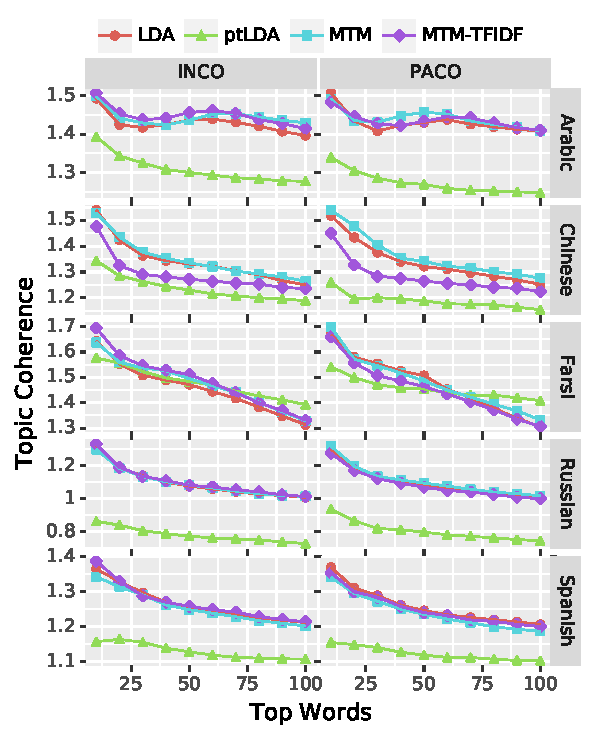
\includegraphics[width=\linewidth]{2019_emnlp_mtm/figures/cv_vertical.pdf}
\caption{Topic coherence on \inco and \paco datasets with the number of top words in each topic.}\label{fig:cv}
\end{figure}

We intrinsically evaluate models' topic coherence on two sets of
preprocessed bilingual Wikipedia corpora~\cite{hao-2018-mtm-doc-link}
that vary in ``nonparallelness''.
%
Both pair English with Arabic, Chinese, Spanish, Farsi, and Russian.
%Each bilingual corpus contains around 2,000 documents
% for both languages.
In \paco, 30\% of documents have direct translations across languages,
and in \inco none has direct translations. Dictionaries are extracted
fromn
Wiktionary.\footnote{\url{https://dumps.wikimedia.org/enwiktionary/}}
Standard preprocessing has already been applied to the datasets,
including stemming, stop word removal, and high-frequency word
removal.
%The first dataset is partially comparable
%(\paco)---30\% of the documents have direct translations in the other
%language. The second one is incomparable (\inco), i.e., no documents
%have direct translations.

\jbgcomment{if there's time, would be good to do posthoc links of LDA
  topics\wycomment{Sorry, this is difficult given my laptop's data loss and the space limit.}}

We use an intra-lingual metric to evaluate topic
coherence~\cite{lau-2014-auto-word-intrusion}: for every topic, we
compute its top~$N$ words' average pairwise \pmi score
on a disjoint subset of Wikipedia
documents~\cite{hao-2018-mtm-doc-link}. We report average
coherence with~$N$ from 10 to 100 with a step size of 10 (five-fold
cross-validation). We use the same translation pair weighting options
as in our classification tasks and also compare against monolingual \lda
and \ptlda~\cite{Hu-2014-ptlda}.

\mtm is no worse than \lda and sometimes slightly
better (Figure~\ref{fig:cv}). \tfidf weighting on translation pairs
sometimes further improves coherence (e.g., Arabic, Farsi,
Russian, and Spanish on \inco) but occasionally hurts (e.g.,
Chinese). \ptlda mostly works poorly, except on Farsi with a high number
of top words. \ptlda aligns topic spaces, which is hard for
low-comparability data, thus sacrificing coherence
for alignment; in contrast \mtm only connects topics when they align well in senses.

\subsection{Topic Coherence vs. Target Language Corpora Sizes}
\label{subsec:topic_link_exp_target_ratio}

\begin{figure}[t]
  \centering
  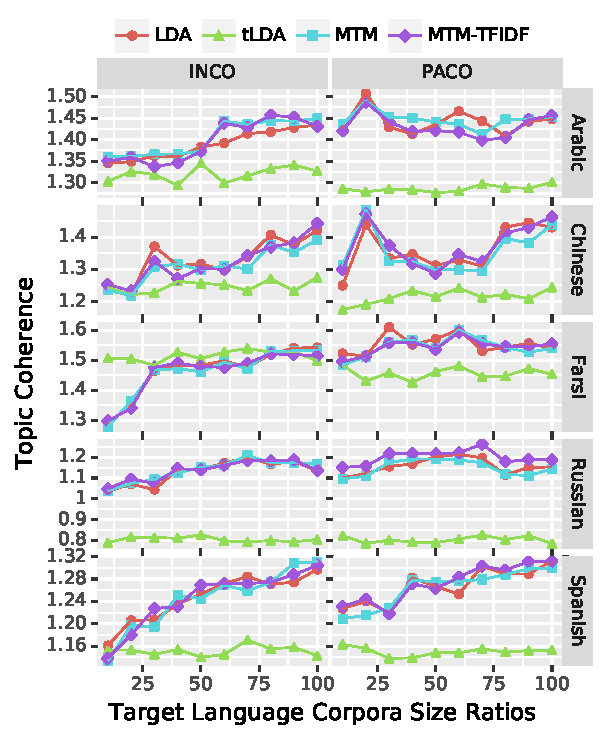
\includegraphics[width=\linewidth]{2019_emnlp_mtm/figures/ratio_vertical.pdf}
  \caption{The models' topic coherence on \inco and \paco datasets
    when the sizes of target language corpora grow from 10\% to 100\%,
    with a step size of 10\%.  \jbgcomment{``performance'' was here;
      make sure you're following style guidelines
      consistently.\wycomment{Done.}}}\label{fig:ratio}
\end{figure}

We next vary the size of target language (non-English languages in
\paco and \inco) corpora: how much can \mtm help topic coherence for
low-resource languages?
%
We start from 10\% of the randomly-selected documents in
target languages and incrementally add more target language documents
at a step size of 10\% until it reaches 100\%.
%
Meanwhile, we always use 100\% of the English documents.
%
We train monolingual \lda, \ptlda, and \mtms with and without \tfidf
weighting on translation pairs on each setting and evaluate the topic
coherence on the same reference corpora using the top thirty words of
each topic (Figure~\ref{fig:ratio}).

In most cases, the topic coherence improves with larger target corpora, except Arabic and Russian on \paco.
%
This confirms our intuition that more data yield a better topic model.
%
\mtm is helpful in cases when the target language corpora sizes are
small, e.g., Chinese and Russian with 10\% or 20\% of the corpora.
%
\tfidf weighting is not consistently better or worse
than equal weights.

The \ptlda with tree priors based on dictionaries performs poorly in
topic coherence, except Farsi in \inco.
%
In most cases, its topic coherence is substantially below others' and
improves little when the target corpora grow.

%\subsection{Target Language Corpus Size}
%\label{subsec:exp_target_ratio}
%
%The experiments are still running, so the results will be added if obtained in time.

%In this section, we study how the sizes of the secondary language corpora affect the topic coherence to simulate the situation when dealing with low-resource languages. In these experiments, we use all of the English documents and vary the size of the secondary language corpora. We randomly create the secondary language corpora by sampling from the original documents and start from 10\% to 100\%, with a step size of 10\%. Then we train a series of \mtms using the English documents and the sampled documents. We run each pair 5 times and report the average topic coherence scores.
%
%The topic coherence scores on the top 100 words given by \lda, \mtm, and \mtm with \tfidf weighting on both~\paco (Figure~\ref{fig:ratio_paco}) and~\inco (Figure~\ref{fig:ratio_inco}) datasets improve as the sizes of the secondary language corpora increase. \mtm, both with and without \tfidf weighting, works slightly better than \lda, although not significantly. \wycomment{Maybe compute the average over all sizes?} The \tlda's performance does not improve with the secondary language corpora sizes. Although it works the best on Farsi, its performance is a lot worse than other models on the rest of the languages.
%
%\begin{figure*}[t]
%\centering
%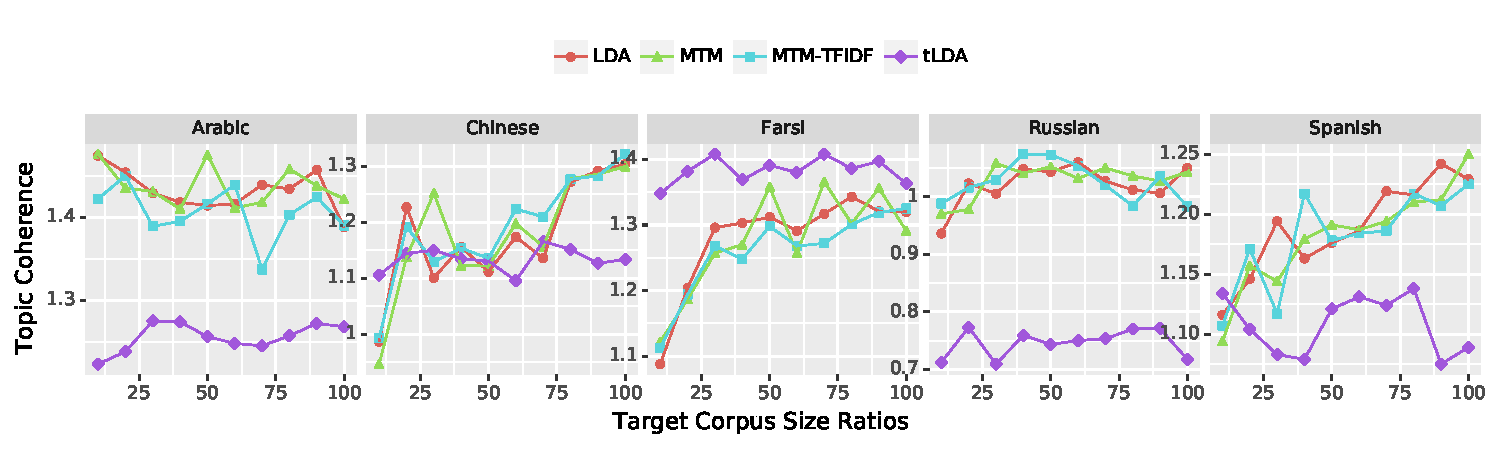
\includegraphics[width=\linewidth]{2019_emnlp_mtm/figures/paco_ratio.pdf}
%\caption{Various target corpus size results on \paco. \wycomment{TODO: Better caption.}}\label{fig:ratio_paco}
%\end{figure*}
%
%\begin{figure*}[t]
%\centering
%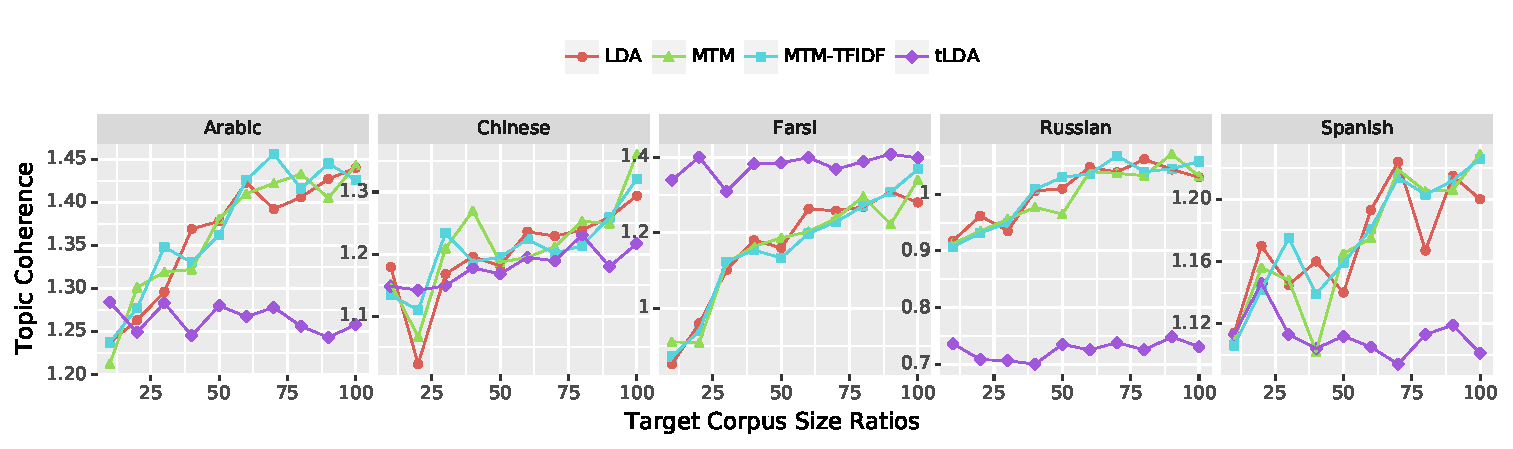
\includegraphics[width=\linewidth]{2019_emnlp_mtm/figures/inco_ratio.pdf}
%\caption{Various target corpus size results on \inco. \wycomment{TODO: Better caption.}}\label{fig:ratio_inco}
%\end{figure*}


%\section{Related Work}
\label{sec:bg}

%Monolingual topic models~\cite{blei-2003-lda} achieve a great success in uncovering latent topics~\cite{griffiths-2004-lda-gibbs} and assisting other downstream tasks, such as information retrieval~\cite{wei-2006-lda-ir}, dialogue segmentation~\cite{purver-2006-dialog-seg}, and even computer vision~\cite{li-2005-tm-cv}.

Monolingual topic models have been extended it to the multilingual case, e.g., analyzing the commonality~\cite{shi-2016-mtm-common} and differences~\cite{gutierrez-2016-mtm-diff} across cultures. 
%
For a multilingual topic model, there must be some external knowledge to bridge the languages. 
%
It could come from document parallelism information, either fully~\cite{mimno-2009-plda} or partially~\cite{hao-2018-mtm-doc-link}. 
%
Another source is the word translations which map words across languages. 
%
Like other prior knowledge, e.g., document links~\cite{daume-2009-mrtf,chang-2010-rtm,Yang:Boyd-Graber:Resnik-2016} and document labels~\cite{ramage-2009-labeled-lda,mcauliffe-2008-slda,zhu-2012-medlda}, word translations can be incorporated in either a \emph{downstream} or an \emph{upstream} way. 
%
A downstream \mtm takes the word translations as supervision and generates them conditioned on the documents, topics, and words~\cite{liu-2015-mtm-downstream}.   \jbgcomment{cite SHLDA, political science-based supervision as well}
%
An upstream \mtm, on the contrary, generates topic assignments conditioned on the word translations~\cite{boyd-graber-2009-muto,jagarlamudi-2010-mtm,boyd-graber-2010-mlslda}. 
%
In addition, tree prior~\cite{boyd-graber-2007-tm-wsd} can also encode
word translations for learning \mtms with tree
\lda~\cite{Hu-2014-ptlda}.

In addition to multilingual topics, multilingual word embeddings have been developed based on monolingual ones~\cite{mikolov-2013-word2vec,pennington-2014-glove} to align semantic dimensions across languages. 
%
Similar to the topic model community, one source of cross-lingual knowledge comes from document alignment, either in whole~\cite{sogaard-2015-mwe-inverted-indexing,hermann-2014-ted} or in part~\cite{vulic-2015-mwe-doc-align}. 
%
Another source is the translation
dictionary~\cite{faruqui-2014-mwe-cca,lu-2015-mwe-deep-cca,ammar-2016-uw-embed},
by projecting two or more semantic spaces into the same one using
canonical correlation analysis~\cite[\cca]{hardoon-2004-cca}.

\jbgcomment{Contrast that embeddings don't give you the high-level
  summaries that you get from topic models.}


\section{Conclusions and Future Work}
\label{sec:conclu}

We introduce a novel multilingual topic model (\mtm) that learns weighted topic links across languages by minimizing the Euclidean distances of translation pairs' (transformed) topic distributions, where translation pairs can be weighted, e.g., by \tfidf.
%
This connects topics in different languages \emph{only} when necessary and is more robust on low-comparability corpora.
%
The \mtm outperforms baselines substantially in both intra- and cross-lingual classification tasks, while achieving no worse or slightly better topic coherence than monolingual \lda on low-comparability data.

We plan to explore weighting methods to better evaluate the importance
of translation pairs.
%
We will also study how to improve topic transformation with the topic
link weight matrices.
% the use of the topic link weight matrices for topic space
% transformation across languages.


\section*{Acknowledgements}

We thank Shudong Hao and Michelle Yuan for providing their datasets. 
%
We thank the anonymous reviewers for their insightful and constructive
comments.
%
This research has been supported under subcontract to Raytheon
\textsc{bbn} Technologies, by \textsc{darpa} award
\textsc{hr}0011-15-\textsc{c}-0113.
%
Boyd-Graber is also supported by \textsc{nsf} grant
\textsc{iis}-1409287.
%
Any opinions, findings, conclusions, or recommendations expressed here
are those of the authors and do not necessarily reflect the view of
the sponsors.


% include your own bib file like this:
\bibliographystyle{style/acl_natbib_2019}
\bibliography{bib/journal-full,bib/wwyang,bib/jbg}

\end{document}
